\documentclass[11pt]{article}
\pagestyle{myheadings}

\usepackage{graphicx}

%------------------------------------------------------------------------------
\newcommand{\stardoccategory}  {Starlink User Note}
\newcommand{\stardocinitials}  {SUN}
\newcommand{\stardocnumber}    {90.9}
\newcommand{\stardocauthors}   {P C T Rees, M J Bly,  P T Wallace}
\newcommand{\stardocdate}      {7 March 1995}
\newcommand{\stardoctitle}     {SNX --- Starlink Extensions to
                                the NCAR Graphics Utilities}
%------------------------------------------------------------------------------

\newcommand{\stardocname}{\stardocinitials /\stardocnumber}
\renewcommand{\_}{{\tt\char'137}}     % re-centres the underscore
\markright{\stardocname}
\setlength{\textwidth}{160mm}
\setlength{\textheight}{230mm}
\setlength{\topmargin}{-2mm}
\setlength{\oddsidemargin}{0mm}
\setlength{\evensidemargin}{0mm}
\setlength{\parindent}{0mm}
\setlength{\parskip}{\medskipamount}
\setlength{\unitlength}{1mm}

%------------------------------------------------------------------------------
% Add any \newcommand or \newenvironment commands here
%------------------------------------------------------------------------------

\begin{document}
\thispagestyle{empty}
DRAL / {\sc Rutherford Appleton Laboratory} \hfill {\bf \stardocname}\\
{\large Particle Physics \& Astronomy Research Council}\\
{\large Starlink Project\\}
{\large \stardoccategory\ \stardocnumber}
\begin{flushright}
\stardocauthors\\
\stardocdate
\end{flushright}
\vspace{-4mm}
\rule{\textwidth}{0.5mm}
\vspace{5mm}
\begin{center}
{\Large\bf \stardoctitle}
\end{center}
\vspace{5mm}

\includegraphics[width=0.95\textwidth]{sun90-fig-1.eps}

\newpage

%------------------------------------------------------------------------------
%  Add this part if you want a table of contents
  \setlength{\parskip}{0mm}
  \begin{small}
  \tableofcontents
  \end{small}
  \setlength{\parskip}{\medskipamount}
  \markright{\stardocname}
%------------------------------------------------------------------------------


\newpage
\section {Introduction}

The NCAR graphics suite (SUN/88) consists of a set of subprograms which
can be used to produce complete graphs in a variety of formats.  The
package has been in wide use for some years; the latest version employs
the ISO standard GKS interfaces for its low-level plotting, giving it
access to all Starlink graphics devices, present and future.

The NCAR routines themselves are thoroughly documented, and just a few
simple calls will produce graphs of excellent appearance.  The package
also provides a high level of flexibility, with dozens of different
details of the plot independently controllable to give exactly the
result required.  However, beginners may be daunted by the mass of
features offered, and unless they take the extreme step of reading the
manual may give up before they realise what the package can do for
them.  This document describes minor extensions which provide more
convenient access to certain features without sacrificing flexibility.

The AUTOGRAPH part of the NCAR suite, used in conjunction with the
Starlink NCAR extensions and the Starlink low level plotting package
SGS (SUN/85), offers an alternative high level system to PGPLOT
(SUN/15) for producing graphs of one variable plotted against another.
All of the Starlink extensions provided within SNX enhance the power of
the facilities provided by AUTOGRAPH and make it more accessible to the
beginner.

Here are some of the things you can do using the facilities described
in this document:

\begin{itemize}

\item Open AUTOGRAPH/SGS/GKS with a single call.

\item Plot a finished graph, with annotation, by means of a single call.

\item Include special characters in graph labels (Greek, subscripts,
mathematical symbols, {\em etc.}).

\item Plot character strings anywhere on the graph.

\item Manage the graphics device display surface via the SGS system of
zones while using AUTOGRAPH to do the plotting.

\item Align the AUTOGRAPH and SGS coordinate systems.

\item Save and restore the state of AUTOGRAPH so that multiple active
plots can be managed.

\item Perform cursor input.

\end{itemize}

See Appendices \ref{demo1_sect}--\ref{demo3_sect} for example programs
demonstrating some of these facilities.


\section {Summary of Calls}

\begin{small}
\begin{description}
\item [CALL SNX\_AGOP] \hfill
\subitem Make AUTOGRAPH/SGS/GKS ready for plotting.
\indexspace
\item [CALL SNX\_EZRXY] ( XDRA, YDRA, NPTS, XLAB, YLAB, GLAB )
\subitem Plot (x,y) data, with labelling, using AUTOGRAPH.
\indexspace
\item [CALL SNX\_AGLAB] ( LNAME, TEXT )
\subitem Set up an AUTOGRAPH label.
\indexspace
\item [CALL SNX\_CHSET] ( I )
\subitem Select one of the two NCAR Roman fonts.
\indexspace
\item [CALL SNX\_AGSAV] ( HEAP )
\subitem Save the state of AUTOGRAPH.
\indexspace
\item [CALL SNX\_AGRES] ( HEAP )
\subitem Restore the state of AUTOGRAPH.
\indexspace
\item [CALL SNX\_TO] ( SORN )
\subitem Switch between NCAR and SGS plotting.
\indexspace
\item [CALL SNX\_AGWV] \hfill
\subitem Make the AUTOGRAPH graph window match the current viewport ($=$ zone
if using SGS).
\indexspace
\item [CALL SNX\_AGCS] \hfill
\subitem Make the current SGS zone world coordinates match the AUTOGRAPH grid
coordinate system.
\indexspace
\item [CALL SNX\_CURS] ( X, Y, N )
\subitem Read a cursor position.
\indexspace
\item [UX $=$ SNX\_AGGUX] ( GX )
\subitem Transform grid X coordinate to user X coordinate.
\indexspace
\item [UY $=$ SNX\_AGGUY] ( GY )
\subitem Transform grid Y coordinate to user Y coordinate.
\indexspace
\item [GX $=$ SNX\_AGUGX] ( UX )
\subitem Transform user X coordinate to grid X coordinate.
\indexspace
\item [GY $=$ SNX\_AGUGY] ( UY )
\subitem Transform user Y coordinate to grid Y coordinate.
\indexspace
\item [CALL SNX\_WRTST] ( XG, YG, STRING, HG, IOR, ICTR )
\subitem Plot a character string.
\end{description}
\end{small}

\section {Linking} \label{link_sect}

\subsection {Use with the UNIX operating system}

\begin{sloppypar} Assuming all Starlink directories have been added to
the environment variables {\tt PATH} and {\tt LD\_LIBRARY\_PATH} (see
SUN/118), then to link a non-ADAM program with SNX and NCAR the command
line would be:  \end{sloppypar}

\begin {quote}
\begin {small}
\begin{verbatim}
% f77 program.o -L/star/lib `snx_link` -o program.out
\end{verbatim}
\end {small}
\end {quote}

This command line will link with the SNX, NCAR and SGS libraries.

Two subroutines provided by SNX exist in other forms elsewhere and
require special handling.  The first gives access to the special fonts
provided by the NCAR routine PWRITX:  it is a Starlink version of the
NCAR subroutine AGPWRT.  The second intercepts and changes the numeric
labels produced by AUTOGRAPH, turning ``.1" and ``$-.5$" into ``0.1"
and ``$-0.5$" {\em etc.}: it is a Starlink version of the NCAR
subroutine AGCHNL.  These routines will be automatically linked by
using {\tt `snx\_link`} if you have called the SNX routine {\tt
SNX\_AGOP}.   If you are using SNX routines as part of an NCAR/SGS mix,
and have not called {\tt SNX\_AGOP} to initialise the graphics system,
you must link with the objects directly:

\begin {quote}
\begin {small}
\begin{verbatim}
% f77 program.o /star/lib/agpwritx.o /star/lib/agchnlz.o \
       -L/star/lib `snx_link` -o program.out
\end{verbatim}
\end {small}
\end {quote}

(It is important to realise that the use of the special fonts will naturally
incur a speed penalty.  Advice on this is given in \S\ref{text_sect}.)

Compiling and linking ADAM applications is discussed in Appendix
\ref{adam_link}.

\subsection {Use with the VAX/VMS operating system}

Non-ADAM programs may be linked with the SNX and NCAR libraries by

\begin{quote}
\begin{verbatim}
$ LINK program, NCAR_DIR:SNX_LINK/OPT, STAR_LINK/OPT
\end{verbatim}
\end{quote}

This command line will link with the SNX, NCAR and SGS libraries.

Compiling and linking ADAM applications is discussed in Appendix
\ref{adam_link}.

\section {Initialising AUTOGRAPH/SGS/GKS}

To make AUTOGRAPH/SGS/GKS ready for plotting, use the Fortran statement

\begin{verbatim}
      CALL SNX_AGOP
\end{verbatim}

The routine asks for the SGS/GKS workstation name via the standard input device
used by NCAR (normally the terminal).
If \verb+<CR>+ or an invalid name is entered, a list of all the current names
is displayed and the request is repeated.
Once SGS/GKS and the workstation have all been successfully opened,
AUTOGRAPH is configured to use the full display surface (in other words
the base SGS zone).
If you don't want the AUTOGRAPH plot to fill the display surface, use the SGS
zone creation routines to select the desired region and then call SNX\_AGWV
(see \S\ref{coord_sect}).


\section {Plotting X against Y with AUTOGRAPH}

To plot a labelled graph of the curve joining (x,y) points given as separate x
and y arrays, the following can be used:

\begin{verbatim}
      CALL SNX_EZRXY( XDRA, YDRA, NPTS, XLAB, YLAB, GLAB )
\end{verbatim}

XDRA and YDRA are real 1-dimensional arrays containing the x and y points
respectively; the integer NPTS is the number of (x,y) values; XLAB, YLAB and
GLAB are character strings giving the three labels (x-axis, y-axis and graph).
Trailing blanks in the labels are ignored.
Greek letters and special symbols can be used by including PWRITX function
codes in the strings (see Appendix \ref{PWRT_sect}) by virtue of linking with 
the Starlink version of AGPWRT (\S\ref{link_sect} and \S\ref{text_sect}).

When using SNX, the format of numeric labels is ``0.4", ``$-0.25$" instead of
the default style used by AUTOGRAPH, ``.4", ``$-.25$", by virtue of linking
with the Starlink version of AGCHNL (\S\ref{link_sect}).
Other control over labelling (character sizes, multiple lines, character
orientation, {\em etc.}) can be achieved by setting the appropriate AUTOGRAPH
parameters and then calling the NCAR routine EZXY directly, and by writing
bespoke versions of the user-replaceable routines AGCHNL and AGUTOL.

NCAR can plot other forms of data: {\em e.g.}\ y array only, multiple curves,
{\em etc.}
These are discussed in the NCAR AUTOGRAPH document -- see EZY, EZMY, EZMXY.

Appendices \ref{demo1_sect}--\ref{demo3_sect} contain several examples of the
use of SNX\_EZRXY.


\section {AUTOGRAPH Labels}

To set up one of the four predefined AUTOGRAPH labels (see \S 2.30 {\em et
seq.} in the AUTOGRAPH document), the following call may be used:

\begin{verbatim}
      CALL SNX_AGLAB( LNAME, TEXT )
\end{verbatim}

LNAME and TEXT are both character strings.
The first character of LNAME is the label name (`R', `L', `B' or `T' for
right, left, bottom, top respectively) and TEXT is the label text.
Trailing blanks are ignored so that the text proper is correctly centred --
for deliberate trailing blanks, use `\$' as an endmark.
Also, PWRITX function codes can be inserted for special characters (see
\S\ref{link_sect} and \S\ref{text_sect}).
For LNAME $=$ `T' or `L', the AUTOGRAPH line number is set to 100; for `B' or
`R', the line number is $-100$.

Illegal LNAME values cause the top label to be set to

\begin {quote}
\begin{verbatim}
'*** AGLAB LABEL ERROR ***'.
\end{verbatim}
\end {quote}

The SNX\_AGLAB routine can be used in conjunction with the AUTOGRAPH facilities.
For example, the following calls will create a 2-line `B' label (beneath the
x-axis), with the second line (numbered $-200$) of character height 0.03 grid
units.
Here, one grid unit is the height of the box within which the curve is
plotted.

\begin{verbatim}
      CALL SNX_AGLAB( 'B', 'This is the first line of text' )
      CALL AGSETC( 'LABEL/NAME.', 'B' )
      CALL AGSETI( 'LINE/NUMBER.', -200 )
      CALL AGSETF( 'LINE/CHARACTER.', 0.03 )
      CALL AGSETC( 'LINE/TEXT.', 'This is the second line of text' )
\end{verbatim}

It is permissible to omit the AGSETC call which specifies the `B' label as
this will have been done already by SNX\_AGLAB.


\section {Control over Text Font and Character Set} \label{text_sect}

An ordinary AUTOGRAPH application program linked only with the NCAR library,
{\em e.g.}

\begin {quote}
\begin{verbatim}
$ LINK PROGRAM, NCAR_DIR:NCAR_LINK/OPT, STAR_LINK/OPT
\end{verbatim}
\end {quote}

on VAX/VMS,
will include the standard version of the routine AGPWRT which uses the GKS
text-drawing facilities.
Extremely flexible control over font, colour, {\em etc.}, is available via GKS
(see \S 2.43 of the AUTOGRAPH document), but NCAR itself contains
some facilities for controlling the text font which many users will find more
accessible, particularly when Greek letters, subscripts and other special
characters are to be included in labels.

To use the NCAR fancy fonts, the application program must be linked with a
special Starlink version of the AUTOGRAPH routine AGPWRT, which has access to
the NCAR PWRITX character drawing routine (\S 3).
When using the Starlink version of AGPWRT, PWRITX function codes can be
included in the character strings in order to switch between various sets of
special characters.
Lower case characters and common punctuation marks are automatically handled;
apostrophe (which is used as the delimiter for the PWRITX codes) is specified
by two consecutive apostrophes.
A choice of two native NCAR character sets is available.
The selection can be made as follows:

\begin{verbatim}
      CALL SNX_CHSET( I )
\end{verbatim}

The integer argument I may be either 1 or 2.
I$=$1 selects the ``duplex" font set and I$=$2 the ``complex" font.
The ``complex" characters (the default) are more ornate and
fussier than the comparatively plain ``duplex" characters.
Only the Roman characters are changed by the SNX\_CHSET call --
not the Greek, {\em etc.}

For precise details of how to construct the PWRITX strings, refer to Appendix
\ref{PWRT_sect}, which includes the program preamble comments describing the
AGPWRITX routine, followed by a plot of the available characters.
The principle is that within the string of ordinary characters, function codes
can be embedded describing changes of font, size and position.
The function codes are delimited by apostrophes.
For example, a label meaning $r^{2}$ could be written using the string
``{\tt r'S'2'N'}''.
The ``{\tt r}" is simply drawn as a lower case ``r"; the ``{\tt 'S'}" is a
function code switching to superscript; the ``{\tt 2}" is then drawn as a small
numeral in the superscript position; and finally the ``{\tt 'N'}" switches back
from superscript to normal.
Though daunting at first, the strings are quite easy to construct and to debug
by trial and error.

As a more complicated
example, the string ``{\tt Area = 'GL'P'R'r'S'2}" will generate a label
equivalent to ``Area $=\pi r^{2}$".
(The apostrophes make for messy Fortran literals; this one would be
``{\tt `Area = ''GL''P''R''r''S''2'}''.)
The first PWRITX function code `GL' selects the Greek Lowercase
font;  P happens to be the source character which generates the
pi;  the next function code `R' switches back to Roman for the
r;  the final code `S' means superscript and draws the power of 2 symbol.
More examples are included in the XYPLOT input file listed in Appendix
\ref{demo1_sect}.

Inevitably, use of the special fonts costs plotting time -- each
character is formed from many line segments, all of which have
to be transmitted to the device.
This is compounded by the relatively high density of
numeric labelling which AUTOGRAPH provides by default.
This speed penalty is an acceptable cost where a publication-quality
plot is being produced on a hardcopy device, but not for
interactive applications requiring frequent and rapid plotting.
Appendix \ref{demo2_sect} describes a demonstration program which
switches between three different character drawing
methods and graph styles to achieve different trade-offs
between speed and appearance.
This involves a special form of the call to AGPWRT, available
only with the AGPWRITX implementation of this routine.
The call is:

\begin{verbatim}
      CALL AGPWRT( 0.0, 0.0, ' ', 0, 0, 0, -100 )
\end{verbatim}

or

\begin{verbatim}
      CALL AGPWRT( 0.0, 0.0, ' ', 0, 0, 0, 100 )
\end{verbatim}

(All the arguments except the last one, ICEN, which must be $\pm100$,
are ignored.)
The $-100$ ICEN value selects character drawing via
the ordinary PWRIT routine, which uses the GKS character drawing
facilities and thus allows control of font, precision, {\em etc.}
The +100 ICEN value selects character drawing via the fancy PWRITX routine.


\section {AUTOGRAPH Save and Restore}

It can sometimes be useful to draw several graphs on one
display frame and then to plot additional material to (or
perform input from) one or more of them later.
This can be accomplished by using the
routines SNX\_AGSAV and SNX\_AGRES, which respectively
save and restore the AUTOGRAPH context.  Thus the sequence:

\begin{verbatim}
      Plot something with AUTOGRAPH
      CALL SNX_AGSAV( HEAP )
      Plot something else with AUTOGRAPH
      CALL SNX_AGRES( HEAP )
\end{verbatim}

will leave AUTOGRAPH in the same state as it was after the first plot.
HEAP is a 1-dimensional real array in which SNX\_AGSAV stores
all of AUTOGRAPH's important variables.
HEAP must currently be at least 2606 elements long;
check the SNX\_AGSAV source for the latest value.
If you wish to save several different AUTOGRAPH states in
one program, several HEAP arrays will of course be required.

When using this facility it will very often be necessary to switch SGS zone
(with SGS\_SELZ) as well as saving and restoring AUTOGRAPH.
When this is done, a call to SNX\_AGWV (\S 9.1) will be needed as well.
See also \S 11.

The NCAR software includes its own AUTOGRAPH save/restore facility (AGSAVE,
AGRSTR).
This uses a scratch file, which means that a state saved in one program can be
restored in another, but does not save the plotting context.
It is thus most useful for plotting successive data sets with the same
AUTOGRAPH parameters rather than (for example) making additions to a graph
plotted earlier, something which is for that matter hard to do with GKS itself.


\section {AUTOGRAPH and SGS Coordinate Systems} \label{coord_sect}

\subsection {Making AUTOGRAPH use the current SGS zone}

AUTOGRAPH can be made to plot within the current GKS viewport as follows:

\begin{verbatim}
      CALL SNX_AGWV
\end{verbatim}

This will cause the AUTOGRAPH graph window (the rectangle which
contains the labels, axes, grid, {\em etc.}) to be coincident with the GKS
viewport. A specially convenient way to set up a GKS viewport is by means of
SGS; a call to SNX\_AGWV following any zone creation or selection call will
cause AUTOGRAPH to arrange its plot within that zone.
The zone may be of any aspect ratio,
with the proviso that labels may overflow very narrow ones.


\subsection {Setting the SGS coordinates to match an AUTOGRAPH plot}

Once AUTOGRAPH has established its plotting strategy (usually
after drawing the graph, or either the background or curve) it
may be necessary to make additions to the plot or to perform input.
This can be done conveniently as follows:

\begin{verbatim}
      Plot the graph with AUTOGRAPH
      CALL SNX_AGCS
\end{verbatim}

The call to SNX\_AGCS sets the extent (in world coordinates) of the
current SGS zone, presumed to cover the AUTOGRAPH graph
window (the rectangular area within which the whole AUTOGRAPH
plot, including labels {\em etc.}, is drawn), so that the AUTOGRAPH
grid window (the rectangular
area within which the curve itself is plotted) has bounds
(0.0,1.0,0.0,1.0).
Thus the world coordinates of
the SGS zone are now AUTOGRAPH grid coordinates.
Clipping requirements may then make it necessary
to create another zone covering just the grid window, but
still with grid coordinates.
This is easily accomplished by:

\begin{verbatim}
      CALL SGS_ZONE( 0.0, 1.0, 0.0, 1.0, IZGW, J )
      CALL SGS_SW( 0.0, 1.0, 0.0, 1.0, J )
\end{verbatim}


\subsection {SGS/AUTOGRAPH coordinate conversions}

For data-related plotting and input, four functions are
provided to perform the necessary coordinate conversions.
The two sets of coordinates are respectively the grid
coordinates (GX,GY) and the user ({\em i.e.}\ data) coordinates (UX,UY).

\begin{quote}
To convert a grid x coordinate to a user x coordinate:

\begin{verbatim}
      UX = SNX_AGGUX( GX )
\end{verbatim}

To convert a grid y coordinate to a user y coordinate:

\begin{verbatim}
      UY = SNX_AGGUY( GY )
\end{verbatim}

To convert a user x coordinate to a grid x coordinate:

\begin{verbatim}
      GX = SNX_AGUGX( UX )
\end{verbatim}

To convert a user y coordinate to a grid y coordinate:

\begin{verbatim}
      GY = SNX_AGUGY( UY )
\end{verbatim}
\end{quote}

The grid coordinates are such that the grid window part of
the AUTOGRAPH graph window has bounds (0.0,1.0,0.0,1.0);
they match the world coordinates for a zone set up with SNX\_AGCS
(see the previous section).

The user coordinates relate to the actual data values
supplied, even though the plotting may have been done with
logarithmic scaling or reversed directions.


\section {Plotting Character Strings}

AUTOGRAPH provides for multiline labels in one of several
predefined regions of the plot, but can be awkward to use for
placing character strings in arbitrary places.
The SPPS routine WTSTR is more suitable for this purpose, but
operates in user ({\em i.e.}\ data) coordinates, not appropriate for
plotting outside the grid window, and expresses the character
size in low level ``plotter units".
Character strings can, of course, be plotted directly
through GKS or SGS, though access to the special NCAR fonts
will not be available.

The Starlink extension routine SNX\_WTRST is a further method
of plotting strings.
The call is as follows:

\begin{verbatim}
      CALL SNX_WRTST( XG, YG, STRING, HG, JOR, JCTR )
\end{verbatim}

XG,YG (real) is the position of the string in grid coordinates.
STRING is the character string to be plotted, and may contain PWRITX codes
(see \S 7) if special characters are required.
This option requires linking with the AGPWRITX
version of AGPWRT (see \S 3).
HG (real) is the character height in grid Y units.
JOR (integer) is the string orientation, in degrees anticlockwise from
the usual left-to-right.
JCTR (integer) describes the justification; $-2$ and $-1$ $=$ left,
0 $=$ centred, +1 and +2 $=$ right, where ``left" means ``the middle of
the left edge of the leftmost character is at XG,YG" {\em etc.}
The values 0 and $\pm2$ produce proportionally-spaced strings and
allow fancy characters to be used;
$\pm1$ produces monospaced strings consisting of ordinary letters
(including lowercase), numbers and punctuation characters.
You would use $\pm1$ for plotting a table -- 
the AUTOGRAPH numeric labels are plotted using this value.
There is no provision for centred monospaced strings.


\section {Mixing GKS, SGS and NCAR Plotting}

Most plotting packages are designed to be used on their own,
and cannot be used in conjunction with any other package.
In contrast, SGS has been designed to permit direct use of
GKS, and it is also possible, with care, to use the NCAR routines
in combination with SGS and GKS very effectively.
However, NCAR and SGS/GKS are separate plotting systems and some
care is necessary when switching back and forth between them.

Two packaged save/restore facilities exist within SNX to help
do this.
The most elaborate is the pair of routines SNX\_AGSAV and SNX\_AGRES
(see \S 8), which are a complete save and restore for AUTOGRAPH.
A simpler facility, which performs the
necessary buffer flushing operations and saves/restores the
SGS zone, is the SNX\_TO routine.
This is used as follows:

\begin{verbatim}
      Plot with NCAR
      CALL SNX_TO( 'SGS' )
      Plot with SGS
      CALL SNX_TO( 'NCAR' )
      More plotting with NCAR
\end{verbatim}

Only the first character of the argument is significant.
The sequence must begin with the switch to SGS and then alternate strictly.

When you have just plotted something using an NCAR
routine (or at least a low level one -- the high level utilities do it
for you) and wish to switch to SGS or GKS, make the following call:

\begin{verbatim}
      CALL PLOTIT( 0, 0, 2 )
\end{verbatim}

or if you are switching from SGS:

\begin{verbatim}
      CALL SGS_FLUSH
\end{verbatim}

or from GKS:

\begin{verbatim}
      CALL GUWK( WKID, REGFL )
\end{verbatim}

After plotting with AUTOGRAPH, further GKS or SGS work will
require the coordinate systems to be re-established.
In SGS this can be done as follows:

\begin{verbatim}
      CALL SGS_ICURZ( IZ )
      CALL SGS_SELZ( IZ )
\end{verbatim}

This can be omitted if the routine SNX\_AGCS is being called.
Conversely, the NCAR coordinate systems will need to be saved and
restored if there is intervening SGS or GKS plotting.
This can be done by means of the SPPS routines
GETSET and SET.


\section {Cursor Input}

To input coordinates from a graph plotted with AUTOGRAPH, use the call

\begin{verbatim}
      CALL SNX_CURS( X, Y, N )
\end{verbatim}

X, Y (real) are user ({\em i.e.}\ data) coordinates.
Their value when the call is made is used to preset the cursor
position (if this is possible on the GKS workstation concerned).
On exit, they are set to the position indicated by the
cursor input operation.
The integer N is the SGS choice, and will generally indicate the button
that has been pressed.

Variations of choice device, cursor visibility, echo type,
{\em etc.}, may be made by direct SGS/GKS calls before SNX\_CURS is called.

Appendix \ref{demo3_sect} contains a demonstration program for SNX\_CURS.


\section {References}

\begin{verse}
SGP/16 ~~Starlink Application Programming Standard.\\
SUN/15 ~~PGPLOT --- Graphics Subroutine Library.\\
SUN/83 ~~GKS --- Graphical Kernel System (7.2).\\
SUN/85 ~~SGS --- Simple Graphics System.\\
SUN/88 ~~NCAR --- NCAR -- Graphics Utilities.\\
SUN/118 ~~Starlink Software on UNIX.\\
SUN/144 ~~ADAM --- UNIX Version.
\end{verse}


\newpage
\appendix
\section {Using SNX within ADAM Applications} \label{adam_link}

\subsection {Use with the UNIX operating system}

\begin{sloppypar}
Assuming all Starlink directories have been added to the environment variables
{\bf PATH} and {\bf LD\_LIBRARY\_PATH} (see SUN/118), then to link an ADAM
application with SNX the command line would be
\end{sloppypar}

\begin{quote}
\begin{verbatim}
% alink application.o `snx_link_adam`
\end{verbatim}
\end{quote}

SUN/144 gives further details of compiling and linking ADAM applications 
with the UNIX operating system.


\subsection {Use with the VAX/VMS operating system}

When developing ADAM applications, all logical names and symbols used 
during compiling and linking are defined by executing the procedures

\begin{quote}
\begin{verbatim}
$ ADAMSTART
$ ADAM_DEV
\end{verbatim}
\end{quote}

The application may then be compiled using the FORTRAN command and linked using
the ALINK and MLINK procedures, {\em e.g.}

\begin{quote}
\begin{verbatim}
$ ALINK application,NCAR_DIR:SNX_LINK_ADAM/OPT
\end{verbatim}
\end{quote}


\section {Portability}

\subsection {Overview}

This section discusses the portability of SNX, including the coding 
standard adopted and a list of those Starlink packages which 
need to be ported to the target machine before a port of SNX can proceed.


\subsection {Coding and porting prerequisites}

The standard of Fortran used for the coding of SNX is fundamentally Fortran 77,
using the Starlink Fortran coding conventions described in SGP/16.
Several common extensions to the Fortran 77 standard are used in the SNX source 
code; they are as follows:

\begin {itemize}
\item symbolic subprogram names may be longer than six characters (but are 
always shorter than ten characters);
\item symbolic subprogram names include the ``\_'' symbol;
\item the full ASCII character set is assumed in character constants.
\end {itemize}

There are no operating system-specific routines in SNX.
SNX requires NCAR, SGS and GKS Vn. 7.2 or GKS Vn. 7.4 to be available.


\section {Demonstration -- the XYPLOT Program} \label{demo1_sect}
 
The following pages contain a listing of the Fortran source for a
program called XYPLOT, plus a sample input file and the plot it
produces.  As well as demonstrating several of the facilities described
in this document, XYPLOT may be useful as a template for developing
other simple graphics utilities, and can be used in its own right as a
convenient way of producing a presentable plot of a list of (x,y)
data.  The Fortran source may be found in the file NCAR\_DIR:XYPLOT.FOR
on VAX/VMS and in the archive {\tt
/star/\-starlink/\-lib/\-snx/\-examples/\-snx-examples\_source.tar} on
UNIX.  On VAX/VMS, this program may be compiled, linked and run using
the command sequence

\begin {quote}
\begin{verbatim}
$ FORTRAN NCAR_DIR:XYPLOT
$ LINK XYPLOT, NCAR_DIR:SNX_LINK/OPT, STAR_LINK/OPT
$ RUN XYPLOT
\end{verbatim}
\end {quote}

On UNIX, this program may already be installed in directory 
{\tt /star/bin/examples/snx}.  If it has been deinstalled and removed to save
space, you can copy the entire source directory to a scratch dircetory, and
with the SYSTEM environment variable set appropriately, build and run it thus:

\begin {quote}
\begin{verbatim}
% setenv SYSTEM alpha_OSF/1
% ./mk xyplot
% ./xyplot
\end{verbatim}
\end {quote}

\sloppypar
XYPLOT reads an input file and plots a graph.  The input file consists
of a sequence of alphanumeric records, the first three of which are the
labels (title, x-axis, y-axis) with the rest each containing an (x,y)
point (in free format).  The example data may be found in the file
NCAR\_DIR:XYPLOT.DAT on VAX/VMS and {\tt
/star/\-bin/\-examples/\-snx/xyplot.dat} on UNIX (if installed).  The
resulting graph consists of a line joining the points in the order in
which they are given.

\subsection {Fortran source}

\small
\begin{verbatim}
      PROGRAM XYPLOT
*+
*     - - - - - - -
*      X Y P L O T
*     - - - - - - -
*
*   Plot xy data from a file using NCAR package.
*
*   Input is from LU 1.  The format is:
*
*           graph label text
*           x label text
*           y label text
*           x y
*           x y
*           x y
*            :
*            :
*
*   P T Wallace   Starlink   May 1987
*
*+
      IMPLICIT NONE

      INTEGER N,NP,NPMAX
      PARAMETER (NPMAX=10000)
      CHARACTER FNAME*80,GLAB*80,XLAB*80,YLAB*80
      REAL X(NPMAX),Y(NPMAX)


*  Open input file
      PRINT *,'Filename?'
      READ (*,'(Q,A)') N,FNAME
      OPEN (UNIT=1,STATUS='OLD',FILE=FNAME(:N),READONLY)

*  Read label text
      READ (1,'(A)',END=100) GLAB
      READ (1,'(A)',END=100) XLAB
      READ (1,'(A)',END=100) YLAB

*  Read x,y data
      DO NP=1,NPMAX
         READ (1,*,END=100) X(NP),Y(NP)
      END DO
      NP=NPMAX+1

*  Adjust number of points
 100  CONTINUE
      NP=NP-1

*  Plot the graph
      IF (NP.GE.2) THEN
         CALL SNX_AGOP
         CALL SNX_EZRXY(X,Y,NP,XLAB,YLAB,GLAB)
         CALL SGS_CLOSE
      ELSE
         PRINT *,'*** Insufficient Data ***'
      END IF

      END
\end{verbatim}
\normalsize

Notice that most of the program is devoted to reading in the data, and that
the plotting itself requires just three calls -- to open, plot and close
respectively.

The reasons SNX\_EZRXY expects you to do the SGS/GKS open and close rather
than providing truly one-call plotting by doing them itself are:

\begin{itemize}
\item you may not want to use SGS
\item you may want to plot within a selected region of the display surface
\item you may want to do more graphics I/O later on in the same program.
\end{itemize}

The trade-off is fractionally less convenience versus greatly
increased versatility.


\subsection {Input file}

The beginning of the file which was used to produce the
graph on the next page is given below.
Note the use of PWRITX function codes in the three label records;
this assumes the program
has been linked with the special version of the AGPWRT
routine (see \S 3 and 7).
Deliberately complicated example labels have been contrived;
most real applications would require just plain
text without PWRITX codes.

\small
\begin{verbatim}
A Bogus Star 'V:-50IGL'Y'H:-80KRU'C  DLT 1986
Wavelength / '.A'
F'GLB'K'NRU' / 10'S'-26'N' erg cm'S'-2'N' s'S'-1'N' '.AS'-1
   4004.000      0.1888006    
   4008.000      0.0000000E+00
   4012.000      0.0000000E+00
   4016.000      0.3046547    
   4020.000      0.3328641    
   4024.000      3.8437031E-02
   4028.000      0.2980890    
             :
             :
             :
             :
\end{verbatim}
\normalsize

XYPLOT is a convenient tool for quickly debugging complicated label strings.
With a text editor, set up a dummy input file consisting of the label string
you want to try out, then two more arbitrary labels and two arbitrary data
points.
Run the XYPLOT program and inspect the x-axis label; if wrong, edit the data
file and try again.


\subsection {The plot}

XYPLOT produced the following graph when the example input file given
in the previous section was used.
Further copies can be obtained by running XYPLOT and replying with the 
name of the example input file to the `Filename?' prompt.

\begin{figure}
\includegraphics[width=0.95\textwidth]{sun90-fig-1.eps}
\end{figure}

\section {Demonstration -- the SPEED Program} \label{demo2_sect}

The following pages contain a listing of the Fortran source for a
program called SPEED, plus a sample input file.  It produces a plot
similar to the one from XYPLOT (Appendix \ref{demo1_sect}).  The SPEED
program demonstrates three different compromises between plotting speed
and quality of result.  The source and a suitable data file (which is
the same format as for XYPLOT) are distributed with the SNX software:
in the directory NCAR\_DIR on VAX/VMS and in the archive {\tt
/star/\-starlink/\-lib/\-snx/examples/snx-examples.tar} on UNIX.

On VAX/VMS, this program may be compiled, linked and run using the command
sequence

\begin {quote}
\begin{verbatim}
$ FORTRAN NCAR_DIR:SPEED
$ LINK SPEED, NCAR_DIR:SNX_LINK/OPT, STAR_LINK/OPT
$ RUN SPEED
\end{verbatim}
\end {quote}

On UNIX, this program may already be installed in directory 
{\tt /star/bin/examples/snx}.  If it has been deinstalled and removed to save
space, you can copy the entire source directory to a scratch dircetory, and
with the SYSTEM environment variable set appropriately, build and run it thus:

\begin {quote}
\begin{verbatim}
% setenv SYSTEM alpha_OSF/1
% ./mk speed
%./speed
\end{verbatim}
\end {quote}


The program will prompt ``Filename?" (respond NCAR\_DIR:SPEED.DAT on VAX/VMS
and {\bf /star/\-starlink/\-lib/\-snx/speed.dat} on UNIX) and ``Workstation?" 
(give the SGS workstation name). 
The prompt:

\begin {quote}
\begin{verbatim}
    Precision/font?  H=h/w, S=GKS, N=NCAR, E=exit
\end{verbatim}
\end {quote}

will then appear.
The three font options are as follows:

\begin{itemize}
\item A response of ``N" selects the fancy NCAR fonts and allows
AUTOGRAPH to determine the numeric labelling density.
The result is of high quality but takes a long time to plot.
\item A response of ``S" selects the GKS default font.
The result is much quicker, and still presentable.
\item A response of ``H" selects the hardware font and requests
a reduced density of numeric labelling.
On devices which have hardware character generation (most do),
the plot is very rapid but may not be especially attractive.
(One common defect is that the y-label may appear reversed, because the
device is unable to plot characters on their sides and yet the
positions of the individual characters are unchanged.)
\end{itemize}


\subsection {Fortran source}

\small
\begin{verbatim}
      PROGRAM SPEED

*+
*
*  Demonstration of different plotting style/speed
*  tradeoffs in NCAR/SGS/GKS
*
*  P T Wallace   Starlink   10 June 1987
*  P C T Rees    Starlink   19 May 1992
*     Replaced FLUSH calls with PLOTIT calls.
*
*+

      IMPLICIT NONE

      INTEGER NPMAX
      PARAMETER (NPMAX=10000)
      INTEGER N,NP,IPREC,NCOUNT
      REAL RNULL1,TICK
      CHARACTER FNAME*80,GLAB*80,XLAB*80,YLAB*80,K*1
      REAL X(NPMAX),Y(NPMAX)
      LOGICAL PLOTED,NTBAD



*  Open input file
      PRINT *,'Filename?'
      READ (*,'(Q,A)') N,FNAME
      OPEN (UNIT=1,STATUS='OLD',FILE=FNAME(:N),READONLY)

*  Read label text
      READ (1,'(A)',END=9000) GLAB
      READ (1,'(A)',END=9000) XLAB
      READ (1,'(A)',END=9000) YLAB

*  Read x,y data
      DO NP=1,NPMAX
         READ (1,*,END=100) X(NP),Y(NP)
      END DO
      NP = NPMAX+1

*  Adjust number of points
 100  CONTINUE
      NP = NP-1

*  Check enough data
      IF (NP.LT.2) GO TO 9000

*  Prepare to plot the graph
      CALL snx_AGOP
      CALL AGGETF('NULL/1.',RNULL1)
      PLOTED = .FALSE.

*  Select character precision and font
 200  CONTINUE
      PRINT *,'Precision/font?  H=h/w, S=GKS, N=NCAR, E=exit'
      READ (*,'(A)') K
      NTBAD = .FALSE.
      IF (K.EQ.'H'.OR.K.EQ.'h') THEN

*     Hardware characters - fast but tacky
         CALL AGPWRT(0.0,0.0,' ',0,0,0,-100)
         IPREC = 0
         NCOUNT = 1
         TICK = 1.0

      ELSE IF (K.EQ.'S'.OR.K.EQ.'s') THEN

*     GKS software characters - reasonably fast and attractive
         CALL AGPWRT(0.0,0.0,' ',0,0,0,-100)
         IPREC = 2
         NCOUNT = 6
         TICK = RNULL1

      ELSE IF (K.EQ.'N'.OR.K.EQ.'n') THEN

*     PWRITX characters - fancy but slow
         CALL AGPWRT(0.0,0.0,' ',0,0,0,100)
         IPREC = 2
         NCOUNT = 6
         TICK = RNULL1

      ELSE IF (K.EQ.'E'.OR.K.EQ.'e') THEN

*     Exit requested - wrap up
         CALL sgs_CLOSE
         GO TO 9999

      ELSE

*     Unrecognised command
         NTBAD = .TRUE.
         PRINT *,'?'

      END IF

*  Repeat prompt if problems
      IF (NTBAD) GO TO 200

*  Clear the zone if necessary
      IF (PLOTED) CALL sgs_CLRZ

*  Setup for plotting:
*
*  SGS/GKS text precision
      CALL sgs_SPREC(IPREC)

*  Density of tick marks and numeric labels
      CALL AGSETI('LEFT/MAJOR/COUNT.',NCOUNT)
      CALL AGSETI('RIGHT/MAJOR/COUNT.',NCOUNT)
      CALL AGSETI('BOTTOM/MAJOR/COUNT.',NCOUNT)
      CALL AGSETI('TOP/MAJOR/COUNT.',NCOUNT)
      CALL AGSETF('LEFT/MINOR/SPACING.',TICK)
      CALL AGSETF('RIGHT/MINOR/SPACING.',TICK)
      CALL AGSETF('BOTTOM/MINOR/SPACING.',TICK)
      CALL AGSETF('TOP/MINOR/SPACING.',TICK)

*  Plot the graph
      CALL snx_EZRXY(X,Y,NP,XLAB,YLAB,GLAB)
      CALL PLOTIT(0,0,2)
      CALL sgs_FLUSH

      PLOTED = .TRUE.

*  Next plot
      GO TO 200

*  Exits
 9000 CONTINUE
      PRINT *,'Insufficient data!'

 9999 CONTINUE

      END
\end{verbatim}
\normalsize


\subsection {Input file}

The beginning of the file which is supplied for use with the
SPEED program is given below.
It is the same format as for the XYPLOT program, but note
that the three label records should not contain
PWRITX function codes as these will not work when
the ``S" or ``H" options are used.

\small
\begin{verbatim}
Simulated Stellar Spectrum
Wavelength
Flux
   5000.000       6.738085    
   5004.000       8.849804    
   5008.000       9.914771    
   5012.000       9.484353    
   5016.000       9.981673    
   5020.000       11.45505    
   5024.000       8.954852    
   5028.000       11.32500    
             :
             :
             :
             :
\end{verbatim}
\normalsize


\section {Demonstration -- the INDEMO Program} \label{demo3_sect}

The following pages contain a listing of the Fortran source for a program
called INDEMO.
It produces a plot of a spiral, with a logarithmic y-axis and an x-axis with
the scale running right to left.
The objective is to demonstrate the SNX\_CURS input routine, and to show that
data coordinates can be read in and used.
Again, the source is distributed with the SNX software: in the directory
NCAR\_DIR on VAX/VMS and {\bf /star/\-starlink/\-lib/\-snx/examples} on UNIX.

On VAX/VMS, this program may be compiled, linked and run using the command
sequence

\begin {quote}
\begin{verbatim}
$ FORTRAN NCAR_DIR:INDEMO
$ LINK INDEMO, NCAR_DIR:SNX_LINK/OPT, STAR_LINK/OPT
$ RUN INDEMO
\end{verbatim}
\end {quote}

On UNIX, this program may already be installed in directory 
{\tt /star/bin/examples/snx}.  If it has been deinstalled and removed to save
space, you can copy the entire source directory to a scratch dircetory, and
with the SYSTEM environment variable set appropriately, build and run it thus:

\begin {quote}
\begin{verbatim}
% setenv SYSTEM alpha_OSF/1
% ./mk indemo
% ./indemo
\end{verbatim}
\end {quote}

Give the SGS workstation name in response to the ``Workstation?" prompt.
The graph will be plotted, and the cursor will appear.
Adjust the cursor position and press the ``hit" key (normally numeric 1 and 2
on the keyboard).
A cross will be drawn at the cursor position, and next
to it a message giving the data coordinates at that point.
The program will exit when a cursor ``hit" is made outside the plot bounds,
or a zero cursor choice entered.


\subsection {Fortran source}

\small
\begin{verbatim}
      PROGRAM INDEMO

*+
*
*     - - - - - - -
*      I N D E M O
*     - - - - - - -
*
*   Demonstrate cursor input following NCAR AUTOGRAPH plot.
*
*   P T Wallace   Starlink   May 1987
*   P C T Rees    Starlink   April 1992
*      Added exit on cursor choice 0.
*
*+

      IMPLICIT NONE

      INTEGER I,N
      LOGICAL LOOP
      REAL V,T,X(1000),Y(1000),XU,YU,XG,YG,XA(1),YA(1)
      CHARACTER S*13

      REAL snx_AGUGX,snx_AGUGY



*  Fill the data arrays.
      XU = 300.0
      YU = 400.0

      DO I=1,1000
         V = REAL(I-1)
         T = V/50.0
         X(I) = XU + V*COS(T)/2.0
         Y(I) = YU + V*SIN(T)/2.5
      END DO

*  Open NCAR/SGS/GKS.
      CALL snx_AGOP

*  X axis is reversed linear.
      CALL AGSETI('X/ORDER.',1)

*  Y axis is logarithmic.
      CALL AGSETI('Y/LOG.',1)

*  Plot the graph.
      CALL snx_EZRXY(X,Y,1000,'Spiral','x','y')

*  Loop - mark positions on plot.
      LOOP = .TRUE.

      DO WHILE (LOOP)

*     Input a cursor position.
         CALL snx_CURS(XU,YU,N)

*     Check cursor choice and finish if zero.
         IF (N.LE.0) THEN

*        Finish.
            LOOP=.FALSE.
         ELSE

*        Transform to grid coordinates.
            XG = snx_AGUGX(XU)
            YG = snx_AGUGY(YU)

*        Inside or outside grid window?
            IF (XG.LE.1.0.AND.XG.GE.0.0.AND.
     :          YG.LE.1.0.AND.YG.GE.0.0) THEN

*           Inside - mark the selected position.
               WRITE (S,'(''('',F5.1,'','',F5.1,'')'')') XU,YU
               XA(1) = XU
               YA(1) = YU
               CALL POINTS(XA,YA,1,-2,0)
               CALL snx_WRTST(XG+0.02,YG,S,0.02,0,-2)
            ELSE

*           Outside - finished.
               LOOP = .FALSE.
            END IF
         END IF

*  Next position
      END DO

*  Wrap up
      CALL sgs_CLOSE

      END
\end{verbatim}
\normalsize


\section {PWRITX} \label{PWRT_sect}

The special version of the AGPWRT routine described earlier uses the
PWRITX routine to plot the required character string.  A feature of
this routine is that function codes can be embedded in the character
string to select different fonts, draw subscripts, {\em etc.} These
function codes are the ones you will need to use if you wish to have
Greek letters, {\em etc.}\ in your labels.  The AGPWRITX documentation
is given below, and is followed by a plot showing all the available
characters (the Roman characters being those in the ``complex" font).

\begin{verbatim}
      SUBROUTINE AGPWRT( XPOS, YPOS, CHRS, NCHS, ISIZ, IORI, ICEN )
\end{verbatim}

This routine is a substitute for the NCAR routine of the
same name, but allowing the PWRITX character drawing routine
to be used instead of the usual PWRIT, giving access to special fonts, 
{\em etc.}

The character string accepted by the PWRITX routine includes
control codes to switch font, {\em etc.} 
This implementation of
AGPWRT accepts and passes PWRITX codes and also inserts the
appropriate codes where lowercase and certain other characters
are supplied.
Some special characters not directly available
from PWRITX are produced by means of control sequences selected
through additional codes which are peculiar to this implementation of AGPWRT.

Other special values of the ICEN parameter are used to select
plotting via either the PWRITX routine or the PWRIT routine.
This feature allows an application to plot using GKS character
drawing facilities on some occasions while using PWRITX on other
occasions.  The PWRITX option gives high quality characters from
a rich set, but slowly;  the GKS option, on the other hand,
provides access to other GKS fonts and allows the use of lower
text precision on graphics devices where this will reduce the
plotting time.

The NCAR utilities use values of the justification argument ICEN
of $\pm1$ where left or right justification is required,
and in these cases the string is plotted artificially monospaced to
avoid irregular axis labelling, subject to the restriction that
the string must not contain PWRITX function codes (though lowercase
and common punctuation symbols are acceptable).  To enable left
and right justified strings to be proportionally spaced and to
contain PWRITX function codes, this implementation of AGPWRT also
supports the non-NCAR values ICEN $=\pm2$.  There is no
provision for centred monospaced strings.

Given:

\begin{tabbing}
XXXX\=XPOS,YPOSxxx\=xxxxxx\=\kill
\>XPOS,YPOS\>r,r\>string position in SPPS user coordinates\\
\>CHRS,NCHS\>c,i\>string and length, inclusive of codes, {\em etc.}\\
\>ISIZ\>i\>character size\\
\>IORI\>i\>orientation\\
\>ICEN\>i\>justification, or PWRIT/PWRITX selection
\end{tabbing}

Where the special values of ICEN are used to select plotting
via either PWRIT or PWRITX, the other arguments are ignored.

Plotter units:

\begin{quote}
Displacements and character sizes are specified in ``plotter units".
(N.B.\ Do not confuse plotter units with device
coordinates.  Plotter units are not related to true device
resolution.)  Normally the longest dimension of the display
surface is 1024 plotter units.  Should the resolution
limitation that this implies be unacceptable, it can be
changed by means of the SPPS routine SETI.
\end{quote}

PWRITX fonts:

\begin{quote}
Twelve fonts are provided, each containing 47 symbols and indexed
by the standard Fortran characters (\verb%A-Z 0-9 +-*/()$=,.% and space).
A given font is specified by three letters which, in broad terms,
select which combination of size (Principal, Indexical,
Cartographic), alphabet (Roman, Greek), and case (upper, lower) is required.
\end{quote}

ISIZ argument:

\begin{quote}
ISIZ specifies an overall magnification factor for all the characters drawn.

Each of the three size classifications in the set of twelve
fonts provided (Principal, Indexical and Cartographic) has a
nominal character width (in spite of proportional spacing),
height and total height.  The space character is exactly one
nominal width wide, and a carriage control code causes
a downwards increment equal to the nominal total height, which
thus includes white space.

The nominal width (W), height (H), and total height (T) for
the Principal (P), Indexical (I), and Cartographic (K) fonts
are as follows (plotter units):

\begin{tabbing}
XXXXXXXX\=XXXXXX\=XXXXXX\=XXXXXX\=\kill
\>\>W\>H\>T\\
\>P\>16\>21\>32\\
\>I\>12\>13\>20\\
\>K\>8\>9\>14
\end{tabbing}

ISIZ values of 3 or less select standard magnifications of the
above sizes.  Values of 4 or more are proportional to the
resulting magnification.  The overall magnification for
different ISIZ values is as follows:

\begin{tabbing}
XXXXXXXX\=XXXXXXXX\=\kill
\>ISIZ\>mag\\
\\
\>$<1$\>8/21\\
\>1\>12/21\\
\>2\>18/21\\
\>3\>24/21\\
\>$>3$\>ISIZ/21\\
\end{tabbing}

Thus, for ISIZ$>$3, Principal characters will be drawn nominally
ISIZ plotter units high, and ISIZ can simply be thought of
as the nominal character height in plotter units.
\end{quote}

IORI argument:

\begin{quote}
IORI is the string orientation in degrees anticlockwise from the normal
left-to-right.
\end{quote}

ICEN argument (normal use to specify positioning):

\begin{quote}
\begin{tabbing}
XXXXXXXX\=\kill
ICEN\>Meaning\\
\\
--2\>(XPOS,YPOS) is the centre of the left edge of the first character.  The\\
\>string is proportionally spaced.\\
\\
--1\>(XPOS,YPOS) is the centre of the left edge of the first character.  The\\
\>string is monospaced.  Lowercase and punctuation characters are permitted,\\
\>but not function codes.\\
\\
0\>(XPOS,YPOS) is the centre of the entire string.  The string is\\
\>proportionally spaced.\\
\\
+1\>(XPOS,YPOS) is the centre of the right edge of the last character.  The\\
\>string is monospaced.  Lowercase and punctuation characters are permitted,\\
\>but not function codes.\\
\\
+2\>(XPOS,YPOS) is the centre of the right edge of the last character.  The\\
\>string is proportionally spaced.\\
\end{tabbing}
\end{quote}

ICEN argument (special use to select string drawing routine):

\begin{quote}
\begin{tabbing}
XXXXXXXX\=\kill
ICEN\>Meaning\\
\\
--100\>Selects PWRIT routine, which gives access to GKS fonts, precision, 
{em etc.}\\
\\
+100\>Selects PWRITX routine, which gives access to special fonts and other
features.
\end{tabbing}

Notes:

\begin{itemize}
\item For ICEN = $\pm100$ the other arguments are ignored.
\item Initially, PWRITX is selected.
\item This inelegant use of the ICEN argument is a consequence
of having to work within the standard AGPWRT call, which
is made directly by the AUTOGRAPH utilities.
\end{itemize}
\end{quote}

Characters available without using function codes:

\begin{quote}
\begin{itemize}
\item All uppercase and lowercase Roman characters, and most common
punctuation symbols are available by including them literally
in the string CHRS.
\item Two consecutive apostrophes causes a single apostrophe to be
drawn -- for example ``\verb+Murphy''s Law+".

Both of these are features of this implementation of AGPWRT and
are not available when directly calling PWRITX.
\end{itemize}
\end{quote}

Function codes:

\begin{quote}
Function codes are sequences of characters, enclosed within
apostrophes, which may (except when ICEN$=\pm1$) be included in the
character string CHRS to change font, case, {\em etc.}\ within the plotted
string.
No punctuation is needed between functions except for a
comma between adjacent numbers;  however, commas may be used between
functions to improve readability.
The following are the only legal
function codes.
Any other characters in a function string will be
ignored except that an error report will be issued and, if more
than 10 errors occur within a string, control will be returned to
the main program without further plotting.
At the start of the
string, size, type, and case are Principal, Roman, and Upper.

FONT ALPHABET

\begin{quote}
\begin{tabbing}
XXXXXXXXX\=\kill
R\>Roman characters, {\em etc.}\\
G\>Greek characters, {\em etc.}
\end{tabbing}
\end{quote}

FONT SIZE (see table, above, under ISIZ)

\begin{quote}
\begin{tabbing}
XXXXXXXXX\=\kill
P\>Principal fonts\\
I\>Indexical fonts\\
K\>Cartographic fonts
\end{tabbing}
\end{quote}

FONT CASE

\begin{quote}
\begin{tabbing}
XXXXXXXXX\=\kill
U or Un\>Upper case.  If U is followed by a number n (not separated by a\\
\>comma) then n characters will be drawn in uppercase and\\
\>subsequent characters will be in lowercase.  The U1 option is\\
\>thus particularly useful for capitalizing sentences.\\
L or Ln\>Lower case.  If L is followed by a number n, then n characters will\\
\>be drawn in lower case and subsequent characters will be in upper\\
\>case.
\end{tabbing}
\end{quote}

SUBSCRIPTS AND SUPERSCRIPTS

\begin{quote}
\begin{tabbing}
XXXXXXXXX\=\kill
S or Sn\>Superscript level.\\
B or Bn\>Subscript level.\\
N or Nn\>Normal level.
\end{tabbing}

When switching from some ``base" character size to super- or
subscripting, the character size will change depending on
the base character size.  Principal base characters will be
subscripted or superscripted with indexical characters, with
a 10 plotter unit shift (scaled in accordance with ISIZ) up
or down.  Indexical and cartographic base characters will be
sub- or superscripted with cartographic characters with a
7 plotter unit shift.

If multiple S or B functions are used, the original base
character is forgotten, and the base is simply the one
preceding the latest S or B.

The case of the indexing characters will generally be the
same as that of the base character unless otherwise specified.
There is one exception: a lower case indexical base will be
super- or subscripted with upper case cartographic, as the
lowercase cartographic font is composed of special characters
rather than letters and numbers.

If S, B or N is followed by a number n, then n characters will
be drawn as specified above, after which character size, case
and position will be reset to that of the base characters.
If n is negative, its absolute value will be used instead;  n
cannot be zero.  Do not overlap level definitions given for a
specified number of characters.

The N option returns character, case and size to that of the
base but maintains the current character position.

\begin{verbatim}
   For example:  'U1'T'S1'EST    will be drawn   e
                                                Tst

           and   'U1'T'S'E'N'ST  will be drawn   e
                                                T st
\end{verbatim}
\end{quote}

DIRECT CONTROL OVER POSITION

\begin{quote}
\begin{tabbing}
XXXXXXXXX\=\kill
Hn, HnQ\>Increment horizontally in the frame.  Hn will shift the present\\
\>X position by n plotter units. HnQ will shift the present X position\\
\>by n nominal character widths.  Positive n shifts to the right, and\\
\>negative to the left.  If n is omitted, a value of 1 is assumed.\\
\\
Vn, VnQ\>Increment vertically in the frame.  Vn will shift the present Y\\
\>position by n plotter units.  VnQ will shift the present Y position\\
\>by n nominal character total heights.  Positive n shifts upwards,\\
\>and negative downwards.  If n is omitted, a value of 1 is assumed.\\
\\
H:n\>Increment along the direction of the string by n percent of the\\
\>nominal character height for Principal characters.  If n is positive\\
\>the shift is rightwards, and if negative the shift is leftwards.\\
\>If n is absent there is no shift.\\
\\
V:n\>Increment at right angles to the direction of the string by n percent\\
\>of the nominal character height for Principal characters.  If n is\\
\>positive the shift is upwards, and if negative the shift is\\
\>downwards.  If n is absent there is no shift.
\end{tabbing}

(Note: these two are nonstandard features peculiar to this
implementation of AGPWRT and not available when PWRITX is
called directly.)

\begin{tabbing}
XXXXXXXXX\=\kill
X or Xn \&\>Set X or Y.  If the X or Y appears without a number n, the\\
Y or Yn\>function will do nothing.  Otherwise, the character coordinate in the\\
\>X or Y direction will be set to the plotter coordinate n, so that\\
\>the next character drawn will have this position in X or Y,\\
\>subsequent characters will be drawn from this position.
\end{tabbing}
(Note: within PWRITX, interactions with the proportional font
and justification logic make these functions hard to use, and
they are not recommended.)
\begin{tabbing}
XXXXXXXXX\=\kill
C\>Carriage return: a carriage return and line feed will be done before\\
\>the next character is plotted. N.B.\ The justification applies to\\
\>the final line.
\end{tabbing}
\end{quote}

DIRECTION

\begin{quote}
\begin{tabbing}
XXXXXXXXX\=\kill
D or Dn\>Write down, rather than across the frame.  If D appears without an\\
\>n or if n=0, all characters will be written down until an `A'\\
\>function is encountered.  If D is followed by a number n, n\\
\>characters will be written down and subsequent characters will be\\
\>written across the frame.  If n is negative, the absolute value of\\
\>n is used instead.\\
A\>Write across: escape from the D option.
\end{tabbing}
\end{quote}

SPECIAL CHARACTERS

\begin{quote}
\begin{tabbing}
XXXXXXXXX\=\kill
.A\>Angstrom unit
\end{tabbing}

For example, to draw a string meaning ``three Angstrom units per
millimetre" we might use:

\begin{verbatim}
      CALL AGPWRT( XPOS, YPOS, '3''.A''/mm', ...
\end{verbatim}
\end{quote}

DIRECT CHARACTER ACCESS

\begin{quote}
\begin{tabbing}
XXXXXXXXX\=\kill
nnn\>Numeric character: character number nnn (octal) will be drawn.
\end{tabbing}
\end{quote}
\end{quote}

Called:  AGGETI, AGSETI, SETER, PWRITX, PWRIT, GTNUM, KUPX, KUPY, CPUX, CPUY

This routine uses characters outside the ANSI Fortran 77 character
set.

\includegraphics[height=0.95\textheight]{sun90-fig-2.eps}

\includegraphics[height=0.95\textheight]{sun90-fig-3.eps}

\includegraphics[height=0.95\textheight]{sun90-fig-4.eps}

\includegraphics[height=0.95\textheight]{sun90-fig-5.eps}

\includegraphics[height=0.95\textheight]{sun90-fig-6.eps}

\end{document}
